\pstart Insgelijks \textit{is 't boomhacken}\protect\index{Sachverzeichnis}{bomen kappen} \textit{best na dat het lang still en droog weder zy geweest, want regen nat het} huyt, \textit{en wind} sluyt \textit{het} selve, zoe \textit{dat het water van} \edtext{\textit{binnen}}{\lemma{\textit{van}}\Afootnote{ \textit{ (1) }\ bin \textit{ (2) }\ \textit{binnen} \textit{ L}}} \textit{niet} uyt zeipern \textit{en kan}. (+ pluvia humectat,ventus claudit, ut aqua difficulter exeat +)\pend \pstart \textit{Wanneer men hout}\protect\index{Sachverzeichnis}{hout} \textit{brant om te} buygen \textit{en het} \edtext{syne}{\lemma{\textit{het}}\Afootnote{ \textit{ (1) }\ sine \textit{ (2) }\ syne \textit{ L}}} \textit{Kool} \edtext{geeft}{\lemma{\textit{Kool}}\Afootnote{ \textit{ (1) }\ geft \textit{ (2) }\ geeft \textit{ L}}}, \textit{is een teken dat wel buygen zal en lenig is, grove Kool} geft steevig (+ steiff +) \textit{en} unbuygsaem \textit{hout}\protect\index{Sachverzeichnis}{hout}. \textit{Wel staet te letten dat wanneer men berk of andere houten}\protect\index{Sachverzeichnis}{hout} of the \textit{schepen}\protect\index{Sachverzeichnis}{schip} \textit{brengt, dat men die 4 of 6} duym \textit{langer neemt als} te \textit{maet} \edtext{\textit{buyten}}{\lemma{\textit{maet}}\Afootnote{ \textit{ (1) }\ tuyten \textit{ (2) }\ \textit{buyten} \textit{ L}}} \textit{om in 't} rond \textit{te meten schijnt te vereisschen, wan 't ander zins men te kort zal schieten}\edlabel{boomenend}. 
[160 r\textsuperscript{o}] Witsen\protect\index{Namensregister}{\textso{Witsen,} Nicolaes 1641\textendash 1717} \textit{schips bow en bestier} pag 323. seqq. \edtext{Donne\edlabel{donnestart}}{{\xxref{donnestart}{donneend}}\lemma{Donne}\Bfootnote{Von Donne bis Hollandois vgl. \textsc{N. Witsen}, \cite{00153}a.a.O., S.~223.}} une relation des vaisseaux\protect\index{Sachverzeichnis}{vaisseau} de la Chine\protect\index{Ortsregister}{China (Chine)} sur le rapport d'une personne qui a est\'{e} dans le pays avec les Ambassadeurs Hollandois\edlabel{donneend}. \edtext{Les\edlabel{lesancresstart}}{{\xxref{lesancresstart}{lesancresend}}\lemma{Les}\Bfootnote{Von Les ancres bis eenige vgl. \textsc{N. Witsen}, \cite{00153}a.a.O., S.~224.}} ancres\protect\index{Sachverzeichnis}{ancre} des Chinois de bois\protect\index{Sachverzeichnis}{bois} qui va \`{a} fonds aussi bien que le meilleur fer. \textit{Dees }\textit{anckers}\protect\index{Sachverzeichnis}{Anker}\textit{ hebben geen }\textit{ankerstocken}\protect\index{Sachverzeichnis}{anker\textendash stokken}\textit{ noch bladen ofte armen op onze wijs, want het onderste van dees }\textit{anckers}\protect\index{Sachverzeichnis}{Anker}\textit{ en is anderst niet als twee stenke uitstekkende }\textit{houten}\protect\index{Sachverzeichnis}{hout}. Ils ont une adresse toute particuliere pour se parler de loin, sans dire un mot \edtext{\textit{waer toe de stier-man}}{\lemma{mot}\Afootnote{ \textit{ (1) }\ want de St \textit{ (2) }\ \textit{waer toe de stier\textendash man} \textit{ L}}} \textit{of Schipper boven op de Schans klimt aen het achter-Casteel}\protect\index{Sachverzeichnis}{achter\textendash kasteel}. \textit{Neemt een stock als een halve} pijk in syn \textit{handen; waer van de helft rot, de helft zwart is geschildert: op het} rammeln \textit{en flaen der} \edtext{\textit{gommen}}{\lemma{\textit{der}}\Afootnote{ \textit{ (1) }\ trommelen \textit{ (2) }\ \textit{gommen} \textit{ L}}} \textit{en trommels}, vangt \textit{hy aen den stock te} zwaejen \textit{en te} zwencken, in velerleye wijsen: \textit{maeckt ook groot misbaer met} zynen \textit{armen} of \textit{handen:} \edtext{[en]}{\lemma{}\Afootnote{er\textit{\ L \"{a}ndert Hrsg. nach Vorlage}}} \textit{dus wert he verstaen van die te Lande, of op} \edtext{\textit{eenige}\edlabel{lesancresend}\edlabel{eenigestart}}{{\xxref{eenigestart}{eenigeend}}\lemma{\textit{eenige}}\Bfootnote{Von eenige bis hebben vgl. \textsc{N. Witsen}, \cite{00153}a.a.O., S.~225.}} \textit{schepen}\protect\index{Sachverzeichnis}{schip}, \textit{welke} insgelijks \textit{op} \edtext{\textit{dese}}{\lemma{\textit{op}}\Afootnote{ \textit{ (1) }\ deese \textit{ (2) }\ \textit{dese} \textit{ L}}} wise \textit{antworden. Door welk middel de Sinesen elkandre van zoo verre men een man kan zien alles konnen doen weten, zonder eenig wort te spreken}. Not ongelijk \textit{hier mee is het doon van te haring-fangers}\protect\index{Sachverzeichnis}{harings\textendash fangers} \textit{in onze see, die} mit \textit{het bewegen van haer muts te kennen weten te geven aen die voorby vaert, hoo veel haring}\protect\index{Sachverzeichnis}{haring} \textit{zy gevangen hebben}\edlabel{eenigeend}. \edtext{Mons.\edlabel{beaucoupstart}}{{\xxref{beaucoupstart}{beaucoupend}}\lemma{Mons.}\Bfootnote{Von Mons. bis beaucoup vgl. \textsc{N. Witsen}, \cite{00153}a.a.O., S.~228.}} Witsen\protect\index{Namensregister}{\textso{Witsen,} Nicolaes 1641\textendash 1717} d'avoir cont\'{e} un jour \`{a} \textit{Amsterdam}\protect\index{Ortsregister}{Amsterdam} \textit{wanneer te meesten ship}\protect\index{Sachverzeichnis}{schip} buyten zyn \textit{en de minste voor ons palen leggen, 663 groote }\textit{ree-Zeils schepen}\protect\index{Sachverzeichnis}{ree\textendash zeils schepen}\textit{ en 586 kleine binne en bylands vaerzuigen}. \edtext{D'o\`{u}}{\lemma{\textit{vaerzuigen}.}\Afootnote{ \textit{ (1) }\ Daraus \textit{ (2) }\ D'o\`{u} \textit{ L}}} il conclut que la quantit\'{e} des vaisseaux \edtext{des villes}{\lemma{}\Afootnote{des villes \textit{ erg.} \textit{ L}}} Chinoises surpasse celle cy de beaucoup\edlabel{beaucoupend}.
\pend 
\pstart \edtext{\textit{De}\edlabel{deheerstart}}{{\xxref{deheerstart}{deheerend}}\lemma{\textit{De}}\Bfootnote{Von De Heer bis du pays vgl. \textsc{N. Witsen}, \cite{00153}a.a.O., S.~230.}} \edtext{\textit{Heer}}{\lemma{\textit{De}}\Afootnote{ \textit{ (1) }\ heere \textit{ (2) }\ \textit{Heer} \textit{ L}}} \textit{Boechiljon}\protect\index{Namensregister}{\textso{Boechiljon}} welcke \textit{lange} jare \textit{het opperste gezag over de Hollanders en hun handel in japan}\protect\index{Ortsregister}{Japan} \textit{heeft} gehad (dit Witsen\protect\index{Namensregister}{\textso{Witsen,} Nicolaes 1641\textendash 1717} pag. 230) \edtext{dit qu'ils}{\lemma{230)}\Afootnote{ \textit{ (1) }\ conte que \textit{ (2) }\ dit qu'ils \textit{ L}}} ont defendu depuis 30 ans, tout le [commerce]\edtext{}{\Afootnote{commercee\textit{\ L \"{a}ndert Hrsg.}}} maritime \edtext{aux japannois vaisseaux,}{\lemma{maritime}\Afootnote{ \textit{ (1) }\ aux leur \textit{ (2) }\ aux japannois vaisseaux \textit{ L}}} \edtext{}{\lemma{}\Afootnote{de sujets japans \textit{ erg. u. gestr.} \textit{ L}}} et le pouuoire aux sujets, de sortir du pays\edlabel{deheerend}. \edtext{\textit{Noit}\edlabel{noitstart}}{{\xxref{noitstart}{noitend}}\lemma{\textit{Noit}}\Bfootnote{Von Noit bis vermine vgl. \textsc{N. Witsen}, \cite{00153}a.a.O., S.~231.}} \textit{komt eenig verw aen dees}\protect\index{Sachverzeichnis}{Schiff!japanisch} \edtext{\textit{schepen} (de japan)}{\lemma{\textit{schepen}}\Afootnote{ \textit{ (1) }\ het \textit{ (2) }\ (de japan) \textit{ L}}} \edtext{le bois}{\lemma{japan)}\Afootnote{ \textit{ (1) }\ het hout\protect\index{Sachverzeichnis}{hout|textit} \textit{ (2) }\ le bois \textit{ L}}} donc on les fait, est \textit{hagel wit}, nomm\'{e} \textit{Fenuki}\protect\index{Sachverzeichnis}{Fenuki},\rule[-10mm]{0mm}{0mm} except\'{e} que le fonds est de Camphre\protect\index{Sachverzeichnis}{camphre} pour empecher que \edtext{les}{\lemma{que}\Afootnote{ \textit{ (1) }\ lers \textit{ (2) }\ les \textit{ L}}} vers c'y attachent, car l'odeur de Camphre\protect\index{Sachverzeichnis}{camphre} ne souffre point de vermine\protect\index{Sachverzeichnis}{vermine}\edlabel{noitend}.
\pend 
\pstart \edtext{Was\edlabel{tieffgehenstart}}{{\xxref{tieffgehenstart}{tieffgehenend}}\lemma{Was}\Bfootnote{Von Was das tieffgehen bis haben w\"{u}rde vgl. \textsc{N. Witsen}, \cite{00153}a.a.O., S.~240.}} das tieffgehen der schiff\protect\index{Sachverzeichnis}{Schiff} betrifft, die von eichenholz\protect\index{Sachverzeichnis}{Eichenholz} gebauet, werden dieffer sincken als die von vueren Holt\protect\index{Sachverzeichnis}{vurehout}, welche beyde arthen von holz\protect\index{Sachverzeichnis}{Holz} meiner undersuchung nach zusammen seyn, wie 50 zu 43, also daß wenn ein Eichenschiff\protect\index{Sachverzeichnis}{Eichenschiff} 10 fuß tieff gehet soll von \edtext{\textit{Vuuren}}{\lemma{von}\Afootnote{ \textit{ (1) }\ vuren \textit{ (2) }\ \textit{Vuuren} \textit{ L}}} \textit{schip}\protect\index{Sachverzeichnis}{vuuren schip} \textit{van} geleiicke gestalt 8$\displaystyle\frac{3}{5}$\rule[-4mm]{0mm}{10mm} foet \textit{diep} gehen.
\pend 
\pstart Ich achte daß ein schiff\protect\index{Sachverzeichnis}{Schiff} so viel gewalt vom strom bekommen soll, als \edtext{soviel}{\lemma{als}\Afootnote{ \textit{ (1) }\ ob \textit{ (2) }\ soviel \textit{ L}}} waßer, als es einnimt gehabt h\"{a}tte.
\pend 
\pstart Notabile: wenn man mit einer großen gewalt gegen ein \edtext{groß}{\lemma{}\Afootnote{groß \textit{ erg.} \textit{ L}}} schiff\protect\index{Sachverzeichnis}{Schiff} st\"{o}ßet wird mans nicht fortbringen, zieht man aber langsam, so wed man ein schiff\protect\index{Sachverzeichnis}{Schiff} fortziehen es sey so \edtext{schwehr}{\lemma{so}\Afootnote{ \textit{ (1) }\ starck \textit{ (2) }\ schwehr \textit{ L}}} als es wolle. Dieweil als dann das crosterzeil\protect\index{Sachverzeichnis}{crosterzeil} hat von forn wegen und einhender zu lauffen so geschehen aus wann das schiff\protect\index{Sachverzeichnis}{Schiff} bewegt werden soll.
\pend 
\pstart Das Centrum gravitatis\protect\index{Sachverzeichnis}{centrum!gravitatis} des schiffs\protect\index{Sachverzeichnis}{Schiff} ist allezeit in einer rechten \edtext{(+ perpendicular +) Lini}{\lemma{rechten}\Afootnote{ \textit{ (1) }\ (+ perpendicular Lini +) \textit{ (2) }\ (+ perpendicular +) Lini \textit{ L}}} mit dem Centro gravitatis\protect\index{Sachverzeichnis}{centrum!gravitatis}\edtext{; so}{\lemma{gravitatis}\Afootnote{ \textit{ (1) }\ des erstere \textit{ (2) }\ ; so \textit{ L}}} das waßer deßen plazen einnimt haben w\"{u}rde\edlabel{tieffgehenend}.\pend \pstart \edtext{Art schiff\protect\index{Sachverzeichnis}{Schiff} zu meßen erfunden von Herrn Joh. Hudde\protect\index{Namensregister}{\textso{Hudde} (Huddenius), Jan 1628\textendash 1704}. Schepen\protect\index{Sachverzeichnis}{schip} en raath der Stadt amsterdam\protect\index{Ortsregister}{Amsterdam}. Ist durch erfahrung gar just befunden worden. 2 personen konnen damit eines schiffes\protect\index{Sachverzeichnis}{Schiff} Last in 2 uhren meßen.}{\lemma{Art}\Bfootnote{Von Art Schiff bis meßen vgl. \textsc{N. Witsen}, \cite{00153}a.a.O., S.~242.}} \edtext{Experiencen\edlabel{experiencenstart}}{{\xxref{experiencenstart}{experiencenend}}\lemma{Experiencen}\Bfootnote{Von Experiencen bis loth vgl. \textsc{N. Witsen}, \cite{00153}a.a.O., S.~245.}} des Herrn Hudde\protect\index{Namensregister}{\textso{Hudde} (Huddenius), Jan 1628\textendash 1704}\edtext{}{\lemma{Herrn}\Bfootnote{Die Wassergewichte bei Witsen ohne Verweis auf Hudde.}}, geben das \edtext{1 fuß}{\lemma{das}\Afootnote{ \textit{ (1) }\ 1 lb \textit{ (2) }\ 1 fuß \textit{ L}}} regen waßer\protect\index{Sachverzeichnis}{Regenwasser} wiegt 45 lb. 29. lot. Y-water\protect\index{Sachverzeichnis}{Y-water} 46 pond 4$\displaystyle\frac{1}{2}$\rule[-4mm]{0mm}{10mm} loth. Texel waßer\protect\index{Sachverzeichnis}{Texel-Wasser} 46 lb. 18 loth\edlabel{experiencenend}.
\pend 
\clearpage
   \vspace{1.0ex}
%   \begin{center}
%   \pstart \noindent
%   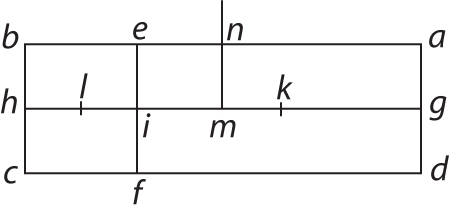
\includegraphics[width=0.3\textwidth]{images/38_160r1}\\{\vrule depth 3.0ex height 0ex width 0mm}
%   \textit{[Fig. 1]}\\
%   $mh\sqcap mg$ \hspace{7mm} \edtext{$\lbrack kl\sqcap mg\rbrack$}{\lemma{}\Afootnote{$kh\sqcap mg$\ \textit{\ L \"{a}ndert Hrsg. }}} \hspace{7mm} $kg\sqcap ki $\\
%   \hspace{20mm}$2km\sqcap ih$ \hspace{3mm} et \hspace{3mm} $km\sqcap il$ \hspace{7mm} $ml\sqcap ik $
%   \pend \end{center} \vspace{-3.0ex}
\pstart Stevini\protect\index{Namensregister}{\textso{Stevin} (Stevinus), Simon 1548\textendash 1620}\edtext{\edlabel{stevinistart}}{{\xxref{stevinistart}{steviniend}}\lemma{Stevini}\Bfootnote{Von Stevini bis demonstrandum erat vgl. \textsc{N. Witsen}, \cite{00153}a.a.O., S.~234.}} beweiß de fundamentali propositione mechanica huc redit: ex solis lineis facile probat esse \edtext{ut}{\lemma{ut}\Bfootnote{Wiedergabe der Figur G der Tafel XCIV, \textsc{N. Witsen, }\cite{00153}a.a.O., nach S.~250, mit Erl\"{a}uterungen auf S.~250 und 251, und Quellenangabe \textsc{Stevin}\protect\index{Namensregister}{\textso{Stevin} (Stevinus), Simon 1548\textendash 1620}, \cite{00196}\textit{Weeg-kunst}, Buch 1.}} \textit{gi} ad \textit{ih}, ita \textit{ml} ad \textit{mk}. Est autem corpus aut pondus \textit{efda}, ad corpus aut pondus \textit{efcb}. Ergo haec erunt ut \textit{ml} ad \textit{mk}. Quod demonstrandum erat\edlabel{steviniend}.
\pend 
\pstart Der\edtext{}{\lemma{Der}\Bfootnote{Von Der große bis gehen vgl. \textsc{N. Witsen}, \cite{00153}a.a.O., S.~253f.}} große mast\protect\index{Sachverzeichnis}{Mast} soll in des schiffs\protect\index{Sachverzeichnis}{Schiff} centrum gravitatis\protect\index{Sachverzeichnis}{centrum!gravitatis}\protect\index{Sachverzeichnis}{centrum!gravitatis|see{centre de gravit\'{e}}} gehen.\pend \pstart \edtext{Große\edlabel{grossestart}}{\lemma{}\Afootnote{Große \textit{ erg.} \textit{ L}}}\edtext{}{{\xxref{grossestart}{grosseend}}\lemma{Große}\Bfootnote{Von Große mast bis 2 mahl vgl. \textsc{N. Witsen}, \cite{00153}a.a.O., S.~254.}} mast\protect\index{Sachverzeichnis}{Mast} soll nicht hoher seyn, als die weite mit der hoehe von schiff\protect\index{Sachverzeichnis}{Schiff} 2 mahl\edlabel{grosseend}.\pend \pstart Witsen\protect\index{Namensregister}{\textso{Witsen,} Nicolaes 1641\textendash 1717} pag. 258. \edtext{Solte\edlabel{gevolgtstart}}{{\xxref{gevolgtstart}{gevolgtend}}\lemma{Solte}\Bfootnote{Von Solte bis gevolgt vgl. \textsc{N. Witsen}, \cite{00153}a.a.O., S.~258.}} iemand fragen warumb der masten\protect\index{Sachverzeichnis}{Mast} getheilt seyn, in 2 oder 3 besondre deilen, und nicht aus einen stick, \edtext{oder}{\lemma{stick,}\Afootnote{ \textit{ (1) }\ so antworte \textit{ (2) }\ oder \textit{ L}}} so die b\"{a}ume nicht hoch genug seyn von sonderlichen st\"{u}cken, mit n\"{a}geln und sonst an einander gef\"{u}get, und zu einem Leichnaem gemacht. Die ursach oder antwort ist, dieweil wenn der mast\protect\index{Sachverzeichnis}{Mast} bestehet aus vielen besonderen deilen, die nur an einander sind festgebunden daß alsdann wann ein st\"{u}ck bricht, das ubrige \edtext{bleibt}{\lemma{ubrige}\Afootnote{ \textit{ (1) }\ ganz bleibt \textit{ (2) }\ bleibt \textit{ L}}}. Item damit man die top-masten\protect\index{Sachverzeichnis}{top-mast} bey harten wetter kan fallen laßen und bey stille wieder heben. \edtext{Dießes}{\lemma{heben.}\Afootnote{ \textit{ (1) }\ Welch \textit{ (2) }\ Dießes \textit{ L}}} ist zu erst erfunden worden 1570 \edtext{durch}{\lemma{1570}\Afootnote{ \textit{ (1) }\ bey \textit{ (2) }\ durch \textit{ L}}} Krijn Wouterß\protect\index{Namensregister}{\textso{Woutersz} (Wouterß), Krijn erw\"{a}hnt 1575}, Schiffer von Enckhuyßen\protect\index{Ortsregister}{Enkhuizen (Enckhuyßen)} \textit{want te voren men de stengen op de groote }\textit{schepen}\protect\index{Sachverzeichnis}{schip}\textit{ woelden aem de toppen de }\textit{masten}\protect\index{Sachverzeichnis}{mast}\textit{ welck stenge schieten naderhand van alle volcken in }\textit{Europa}\protect\index{Ortsregister}{Europa}\textit{ na is gevolgt\edlabel{gevolgtend}}.\pend \pstart \edtext{Ancker\protect\index{Sachverzeichnis}{Anker}\edlabel{anckerstart}}{{\xxref{anckerstart}{anckerend}}\lemma{Ancker}\Bfootnote{Von Ancker bis bequaem vgl. \textsc{N. Witsen}, \cite{00153}a.a.O., S.~259.}} probe, ob sie im grund wohl faßen sollen ist dieße: daß man auff eben grund den punct von einem arme, mit dem ende vom stock auff die erde legt, \textit{zoo het }\textit{ancker}\protect\index{Sachverzeichnis}{Anker}\textit{ met de punct om hoog falt 't is bequaem\edlabel{anckerend}}.\pend \pstart \edtext{Das\edlabel{ruderstart}}{{\xxref{ruderstart}{ruderend}}\lemma{Das}\Bfootnote{Von Das ruder bis waßer vgl. \textsc{N. Witsen}, \cite{00153}a.a.O., S.~260.}} ruder\protect\index{Sachverzeichnis}{Ruder} darf nicht hoher seyn als das waßer kommen kan zu schlagen. \edtext{Noch \textit{lager als}}{\lemma{Noch}\Afootnote{ \textit{ (1) }\ tieffer \textit{ (2) }\ \textit{lager} \textit{ L}}} des konstabels kammer noch tieffer als des Schiffs\protect\index{Sachverzeichnis}{Schiff} Kiel\protect\index{Sachverzeichnis}{Kiel}. Es ist unten breter als oben, weil die untere breite stets unter waßer\edlabel{ruderend}. \edtext{Man\edlabel{winckelstart}}{{\xxref{winckelstart}{winckelend}}\lemma{Man}\Bfootnote{Von Man kan bis winckel vgl. \textsc{N. Witsen}, \cite{00153}a.a.O., S.~261.}} kan nicht wohl weitlauftige regeln geben wie man das ruder\protect\index{Sachverzeichnis}{Ruder} drehen soll, umb \edtext{in}{\lemma{umb}\Afootnote{ \textit{ (1) }\ en 't \textit{ (2) }\ in \textit{ L}}} gegeben streich oder plagam zu fahren. Dieweil bey wenig fortgang und schlappe \textit{stroom die langs} schepes \textit{van} vorn \textit{komt}, \textit{men grooter} hoecken \textit{met het roer}\protect\index{Sachverzeichnis}{roer} \textit{moet maeken, om door het dwars}-setten deßelben mehr kraft von waßer zu faßen, und bey gevolg mehr und genugsamer macht zu bekommen umb das schiff\protect\index{Sachverzeichnis}{Schiff} umb zu sezen. Hingegen bey harten strom und großen vortgang, is wenig \textit{schuinte des} \edtext{\textit{stuurs}}{\lemma{\textit{des}}\Afootnote{ \textit{ (1) }\ Steyers \textit{ (2) }\ \textit{stuurs} \textit{ L}}} genug umb ein schiff\protect\index{Sachverzeichnis}{Schiff} zu versetten (+ umbzutrehen +) dieweil als dann \textit{weinig} waßer große kraft hat. Dahehr der ruder-man\protect\index{Sachverzeichnis}{ruder\textendash man} stets mit den stock in der hand und niemals still stehet dieweil strom umd wind \textit{gestadig bewegen}. Dazu die See \textit{golven} (+ currenten +) die das schiff\protect\index{Sachverzeichnis}{Schiff} umbwerfen, viel thuen. Es wiurde bequem Steuern seyn, wenn das schiff\protect\index{Sachverzeichnis}{Schiff} nur allein von winde auf einen stillen waßer bewegt wurde. Der \textit{stroom} kan [das]\edtext{}{\Afootnote{da\textit{\ L \"{a}ndert Hrsg.}}} Schiff\protect\index{Sachverzeichnis}{Schiff} nicht helffen, als wenn er \textit{recht} uit, oder \textit{naestenby, met het schip}\protect\index{Sachverzeichnis}{schip} \textit{gaet}. Der streit zwischen \textit{Roer}\protect\index{Sachverzeichnis}{roer} (+ Steuer\protect\index{Sachverzeichnis}{Steuer} +) und \edtext{Wind}{\lemma{und}\Afootnote{ \textit{ (1) }\ Vind \textit{ (2) }\ Wind \textit{ L}}}, macht das das schiff\protect\index{Sachverzeichnis}{Schiff} recht aus den streich (+ plagam +) nimt. Denn wenn der wind das schiff\protect\index{Sachverzeichnis}{Schiff} nach osten treibt, und das Ruder\protect\index{Sachverzeichnis}{Ruder} selbigen nach westen tracht zu bringen (+ \Denarius\ \Denarius\ +) soll das schiff\protect\index{Sachverzeichnis}{Schiff} den mittel weg kiesen, und recht aus lauffen nach suden oder Norden (+ hinc patet aliquid aliud necessarium, dann warumb mehr nach suden als norden +). Und das ist die ursach warumb man mit halben wind koers\protect\index{Sachverzeichnis}{koers} en \textit{streeck kan} halten. Dießes hat auch statt, ob man schohn mit einen wind so weit scharffer als halber wind seegelt. Dieße seegel\protect\index{Sachverzeichnis}{Segel} werden absonderlicher weise gestellet, nachdem der wind wehet. Ists halber wind oder noch harter als halber wind, werden die seilen\protect\index{Sachverzeichnis}{Segel} nahe \textit{de achtersteven}\protect\index{Sachverzeichnis}{achtersteven} so \textit{getrocken, over} de seite da der wind hin wehet, und man f\"{u}hrt sie ein wenig nach vorn zu, an die seite da der wind hehr komt damit also der wind schieff an die segel\protect\index{Sachverzeichnis}{Segel} fallende, \textit{het schip}\protect\index{Sachverzeichnis}{schip} \textit{doe draeien tegen} de wind \textit{op, na de} wijse \textit{der molen}-\edtext{\textit{wieken}}{\lemma{\textit{molen-}}\Afootnote{ \textit{ (1) }\ wijcken \textit{ (2) }\ wieken \textit{ (3) }\ \textit{wiecken} \textit{ L}}} den fortgan\protect\index{Sachverzeichnis}{Schiff-Bewegung}, den das schiff\protect\index{Sachverzeichnis}{Schiff} also bekomt, bringt der wiederumb \textit{stuitende} wind zuwege der schieff-eckig auffs seegel\protect\index{Sachverzeichnis}{Segel} falt, und etwas seiner bewegung den seegeln\protect\index{Sachverzeichnis}{Segel} \"{u}bergiebt. Die Schiff\protect\index{Sachverzeichnis}{Schiff} sind ungehorsam den Ruder\protect\index{Sachverzeichnis}{Ruder}, oder \edtext{thun}{\lemma{}\Afootnote{thun \textit{ erg.} \textit{ L}}} \textit{naer} dem \textit{Roer}\protect\index{Sachverzeichnis}{roer} \textit{niet} \edtext{\textit{luisteren}}{\lemma{\textit{niet}}\Afootnote{ \textit{ (1) }\ luijsteren \textit{ (2) }\ \textit{luisteren} \textit{ L}}}; wenn der \textit{stroom} von der seite den fortgang\protect\index{Sachverzeichnis}{Schiff-Bewegung} \textit{recht} aus \"{u}bertrifft, oder wann das \edtext{ruder}{\lemma{das}\Afootnote{ \textit{ (1) }\ rohr \textit{ (2) }\ ruder \textit{ L}}} zu schmahl, keinen waßers lauf genug faßen kan, umb das schiff\protect\index{Sachverzeichnis}{Schiff} zu \textit{bewegen}, item bey stille ohne \textit{stroom}, item ins gemein, wann das ruder\protect\index{Sachverzeichnis}{Ruder} den schiff\protect\index{Sachverzeichnis}{Schiff} nicht wohl proportionirt. (+ even gemaßiget +). Item wann das schiff\protect\index{Sachverzeichnis}{Schiff} hinten nicht genugsam kielet oder sincket, als n\"{o}thig zum waßerfank, item wan es hinten zu breit und das waßer nach nothdurfft gegen das ruder\protect\index{Sachverzeichnis}{Ruder} nicht schl\"{a}gt. Es ist clar, daß ie großer der winckel\edlabel{winckelend} den \edtext{das\edlabel{bepaeltstart}}{{\xxref{bepaeltstart}{bepaeltend}}\lemma{das ruder}\Bfootnote{Von das ruder bis bepaelt. vgl. \textsc{N. Witsen}, \cite{00153}a.a.O., S.~262.}} ruder\protect\index{Sachverzeichnis}{Ruder} mit den kiel\protect\index{Sachverzeichnis}{Kiel} mus machen, so schw\"{a}cher ist der nuzliche (+ vortr\"{a}gliche +) fortgang vom schiff\protect\index{Sachverzeichnis}{Schiff-Bewegung}. Denn es ist ein Zeichen von stille oder gegenwind, und daß wenig oder kraftlooß waßerstroem gegen das ruder\protect\index{Sachverzeichnis}{Ruder} komt zu schlagen. [Bey]\edtext{}{\Afootnote{Bry\textit{\ L \"{a}ndert Hrsg. } }} den schiffen\protect\index{Sachverzeichnis}{Schiff} die zu amsterdam\protect\index{Ortsregister}{Amsterdam} von pferden \"{u}ber straß gezogen werden wenn darhinten etwas fest ist, so ihren lauff \textit{bepaelt}, kan man den Steuer \protect\index{Sachverzeichnis}{Steuer}vergleichen. Denn die geringste bewegung mit einem fuß oder anders, den \edtext{lauff \edlabel{bepaeltend}bepaelt}{\lemma{lauff}\Afootnote{ \textit{ (1) }\ endert \textit{ (2) }\ bepaelt \textit{ L}}}. \pend \pstart \edtext{Das\edlabel{unterworffenstart}}{\lemma{bepaelt.}\Afootnote{ \textit{ (1) }\ Een \textit{ (2) }\ Das \textit{ L}}}\edtext{}{{\xxref{unterworffenstart}{unterworffenend}}\lemma{Das schiff}\Bfootnote{Von Das schiff bis unterworffen vgl. \textsc{N. Witsen}, \cite{00153}a.a.O., S.~265.}} schiff\protect\index{Sachverzeichnis}{Schiff} ist vorn breiter als hinten, dieweil wenn es hinten breiter \edtext{\textit{naer}}{\lemma{breiter}\Afootnote{ \textit{ (1) }\ were \textit{ (2) }\ naer \textit{ L}}} \textit{geen roer en luistert te veel zog} macht, und den fortgang\protect\index{Sachverzeichnis}{Schiff-Bewegung} verhindert, auf den waßer also thut \edtext{\textit{zacken}}{\lemma{thut}\Afootnote{ \textit{ (1) }\ sack \textit{ (2) }\ \textit{zacken} \textit{ L}}}, \textit{dat schier} nichts gegen \textit{'t roer}\protect\index{Sachverzeichnis}{roer} bliyve \textit{waer over} dergleichen schiffs\protect\index{Sachverzeichnis}{Schiff} des schlingern achter sehr unterworffen\edlabel{unterworffenend}.\pend \pstart 